\documentclass[conference]{IEEEtran}
\IEEEoverridecommandlockouts

\usepackage{cite}
\usepackage{amsmath,amssymb,amsfonts}
\usepackage{algorithmic}
\usepackage{graphicx}
\usepackage{textcomp}
\usepackage{xcolor}
\usepackage{kotex}
\def\BibTeX{{\rm B\kern-.05em{\sc i\kern-.025em b}\kern-.08em
    T\kern-.1667em\lower.7ex\hbox{E}\kern-.125emX}}
    
\begin{document}

\title{Connect to parent – FAFA\\ \LARGE(communicate tool for kids via voice recognition)}

\author{\IEEEauthorblockN{Park Hyeong Jin\\2016026271}
\IEEEauthorblockA{\textit{Dept. of Information System}\\ 
\textit{College of Engineering}\\
\textit{Hanyang University}\\
Seoul, Rep. of Korea\\
jin5378@hanyang.ac.kr}
\and
\IEEEauthorblockN{Lee Jun Seok\\2016026444}
\IEEEauthorblockA{\textit{Dept. of Information System}\\ 
\textit{College of Engineering}\\
\textit{Hanyang University}\\
Seoul, Rep. of Korea\\
junslee0912@gmail.com}
\and
\IEEEauthorblockN{Lee Jeong Seon\\2016026435}
\IEEEauthorblockA{\textit{Dept. of Information System}\\ 
\textit{College of Engineering}\\
\textit{Hanyang University}\\
Seoul, Rep. of Korea\\
com2769@gmail.com }
\and
\IEEEauthorblockN{Yoon Seung Gwon\\2016026371}
\IEEEauthorblockA{\textit{Dept. of Information System}\\ 
\textit{College of Engineering}\\
\textit{Hanyang University}\\
Seoul, Rep. of Korea\\
csyoon1472@gmail.com}
}

\maketitle

\begin{abstract}
FAFA is an artificial intelligence speaker based service for two-way communication between children and parents. While the penetration rate of mobile phones in the upper grades of elementary school and above is increasing, the penetration rate of fixed line telephones in the home and those of preschoolers is decreasing. In other words, the isolation of communication means for preschoolers has deepened.

To solve this problem, we developed FAFA which provides two-way communication between parents and children by using artificial intelligence speaker rather than smartphone. Children communicate with each other through NUGU(AI speaker of SKT), and parents through mobile applications. 

\end{abstract}

\section{Introduction}
\subsection{Motivation}
 According to a report by the Korea Information Society Development Institute in 2018, the penetration rate of mobile phones for senior elementary school students is more than 90\%, but the gap is expected to be greater if the penetration rate of lower grades is 58.4\% and kindergarteners are included. In addition, the penetration rate of landline telephones ha been on the decline every year, hitting a record low of 51.9\% in 2019. Through this, the number of children who are left alone at home without a smartphone is increasing without means are not available to contact their parents.
 
 Also, ‘Zenly’, a smartphone application that share the location of friends and family, has been popular with children. We confirmed that there is a strong demand for location sharing services.

\subsection{Problem statement}
There is also a way to open up a child’s smartphone, but parents hesitate to buy it due to the burden of costs and concerns over their young children’s game addiction.

In addition, there are many LBS(Location-Based Service) on the market where parents check their children’s locations, but on the contrary, there is no way for kids left alone at home to get current information about their parents.

\subsection{Solution}
Using SKT’s artificial intelligence speaker NUGU, We developed a two-way connection service for parents and kids without smartphone. A kid left alone at home will be able to interact with their parents in both directions by asking their parents’ location on the speaker. And the parents will be able to check with the application whether the child has arrived home or found themselves.

Since children can use NUGU speakers without the burden of purchasing smartphones, parents do not have any burden on their children’s cell phone addiction and mobile phone costs. In addition, most existing LBS provide one-way communication for parents to connect their kids. But FAFA has a different point in providing two-way communication for parents and kids.

\subsection{Research on any related software}
\begin{enumerate}
    \item Zenly\\
    Zenly is a location-sharing smartphone app that lets you know about your friend and family. Through the app, you can check where and what your friend is doing, and the battery condition or your friend’s cell phone that you cannot reach. You can also know that your friends are at home, at school, on work, or off work.\\
    \item iSharing Lifestyle\\
iSharing by iSharingSoft is an app that provides a real-time locator service allowing family members and close friends to privately share their location information and communicate with each other. iSharing help parents and caregivers reduce anxiety around the whereabouts of their loved ones with easy tracking and alerting messages. There are four main functions.
\begin{enumerate}
    \item Place alert : receive real-time alerts when family arrive at or leave destination
    \item Panic alert : Just shake phone to send notification messages to your family member
    \item Walkie-Talkie : Turn your phone into a Walkie-Talkie.
    \item Location History : See the location history of family member\\
\end{enumerate}
\item NUGU call\\
'NUGU-to-NUGU Call' is service about talking to your NUGU device or NUGU call subscriber.
This call is linked to data. You can use ‘normal mode’ to non NUGU call subscriber. A phone call is linked through the mobile phone of the account connected to the NUGU device.\\
\item NUGU SOS\\
 SOS service is that sends pre-set text messages to designated recipients. You can set the sender's and recipient's information and the emergency SOS message to be sent. If you request an emergency SOS to the NUGU speaker, we will send an emergency SOS message to your registered number.\\
\end{enumerate}

\begin{table}[htbp]
\begin{center}
\caption{Role Assignments}
\begin{tabular}{|c|c|c|}
\hline
Roles & Name & Task description and etc \\ \hline
User  & \begin{tabular}[c]{@{}c@{}} Lee\\Jun Seok \end{tabular}& 
\begin{tabular}[c]{@{}c@{}}Predict what users need from the\\ perspective of a user. Also, consider\\ whether the service is easy to use and\\efficient to use.
If not, find the solution\\ and improve service quality.
\end{tabular}\\\hline

Customer&\begin{tabular}[c]{@{}c@{}}Lee\\Jeong Seon\end{tabular} &  
\begin{tabular}[c]{@{}c@{}}Analyze a service from the perspective\\of a buyer. Also, design service at an\\acceptable cost of money and resource,\\ and focus on cost-effectiveness\\ for raising purchase desire.  \end{tabular}\\ \hline

\begin{tabular}[c]{@{}c@{}}Software\\Developer\end{tabular}&
\begin{tabular}[c]{@{}c@{}}Park\\ Hyeong Jin\end{tabular}&
\begin{tabular}[c]{@{}c@{}}Design overall software to satisfy\\ users and customers' needs. Focus\\ on easiness of design, maintain, and\\reuse its parts.
  \end{tabular}\\ \hline

\begin{tabular}[c]{@{}c@{}}Development\\manger\end{tabular}&
\begin{tabular}[c]{@{}c@{}} Yoon\\Seung Gwon\end{tabular}&
\begin{tabular}[c]{@{}c@{}} Schedule overall project plan and\\ assign the tasks to the members.\\Try to sell more and please customers\\ while costing less to develop\\and maintain.  \end{tabular}\\ \hline  

\end{tabular}
\end{center}
\end{table}

\section{Requirements}
\subsection{AI Speaker}
\begin{enumerate}
    \item Ask parent’s location via voice
    \begin{enumerate}
        \item Set expected utterance, entity and synonym that kid’s intent is asking parent’s location. NUGU play will handle this using STT function.
        \item  Request parent’s location to backend proxy\\
    \end{enumerate}
    \item Answer parent’s location via voice
    \begin{enumerate}
        \item Link user’s intent and action. And configure branch actions according to parent’s location.
        \item Create answer based on Parameters from back-end proxy server and user’s utterance.
        \item NUGU play will answer via voice using TTS function. Set expected utterance that kid’s intent is asking parent’s location.\\

    \end{enumerate}
    \item Send alert to parent
    \begin{enumerate}
        \item Send request to back-end proxy when kids find their parents or tell speaker that they get home
        \item Server keep these request logs in database\\
    \end{enumerate}
    \item Inform that child has arrived home via voice
    \begin{enumerate}
        \item Set expected utterance, entity that kid’s intent is informing that they arrived home. NUGU play will handle this using STT function.
        \item Send request to back-end proxy server to make log.\\
    \end{enumerate}
\end{enumerate}

\subsection{Application (for parent)}
\begin{enumerate}
    \item Sign-in
    \begin{enumerate}
        \item To identify users, user’s ID is required\\
    \end{enumerate}
    \item Set location of home and company
    \begin{enumerate}
        \item To judge parent’s location and status, Parents should set longitude and latitude of home and company.
        \item User could set marker on map using specified button.\\
    \end{enumerate}
    \item Update present location
    \begin{enumerate}
        \item Send recent location data to back-end server automatically every 100 meters.\\
    \end{enumerate}
    \item View kid’s request log
    \begin{enumerate}
        \item Get kid’s request log data from back-end server.
        \item Display the data on page.\\
    \end{enumerate}
\end{enumerate}

\subsection{Server}
\begin{enumerate}
    \item Judge parent’s current location
    \begin{enumerate}
        \item Get parent’s location data from application.
        \item Check latest location and judge status using Machine Learning.
        \item Send result to NUGU play.\\
    \end{enumerate}
    \item Send data to database
    \begin{enumerate}
        \item Server get data from NUGU speaker and application.
        \item Server keep these data in database.
    \end{enumerate}
    \item Make json for NUGU
    \begin{enumerate}
        \item Server should make json file. NUGU speaker demand data in REST API form.\\
    \end{enumerate}
\end{enumerate}

\section{Development Environment}
\subsection{Software Development Platforms}
We chose native app to develop our project, and server acts as REST API. Web environment could also send location data, but we need more precise data and want it to be updated automatically using native app’s background function. React Native which is front-end framework is used. Django which is back-end framework is used for developing REST API to connect with NUGU play.

In addition, we use AWS commercial cloud service such as Elastic Beanstalk for deploy. Lastly, SKT’s NUGU API will be used to analyze kids’ utterance and to recognize their intent. 
\begin{enumerate}
    \item React Native\\
    React Native is a JavaScript framework for writing real, natively rendering mobile applications for iOS and Android. It’s based on React, Facebook’s JavaScript library for building user interfaces, but instead of targeting the browser, it targets mobile platforms. Similar to React for the Web, React Native applications are written using a mixture of JavaScript and XML-esque markup, known as JSX.\\
    \item Django (web framework)\\
    Django is a Python-based free and open source web framework that follows the model-template-views(MTV) architectural pattern. It is maintained by the Django Software Foundation. Django's primary goal is to ease the creation of complex, database-driven websites. The framework emphasizes reusability and "pluggability" of components, less code, low coupling, rapid development, and the principle of don't repeat yourself. Python is used throughout, even for settings files and data models.\\
    
    \item SQLite\\SQLite is a relational database management system (RDBMS) contained in a C library. In contrast to many other database management systems, SQLite is not a client–server database engine. Rather, it is embedded into the end program. SQLite is a popular choice as embedded database software for local/client storage in application software such as web browsers. It is arguably the most widely deployed database engine, as it is used today by several widespread browsers, operating systems, and embedded systems (such as mobile phones), among others. SQLite has bindings to many programming languages.\\
    
    \item Amazon Web Service Elastic Beanstalk(EB)\\
    AWS Elastic Beanstalk is an orchestration service offered by Amazon Web Services for deploying applications which orchestrates various AWS services, including EC2, S3, Simple Notification Service (SNS), CloudWatch, autoscaling, and Elastic Load Balancers. Elastic Beanstalk provides an additional layer of abstraction over the bare server and OS; users instead see a pre-built combination of OS and platform.\\
    
    \item SKTelecom NUGU API\\
    Based on SK Telecom’s technical skills such as voice recognition, voice synthesis and understanding of natural language through NUGU developers, the company can develop new functions through voice command in devices or applications owned by its affiliates. We will recognize and categorize the user’s voice commands through the NUGU API and send output results to the user via voice.\\
    
    \item Google Maps API\\
    The Google Map API provides a variety of functions to produce map-based services on Web (Javascript) and mobile applications (Android, iOS). Local API provides contents and data of Google Map through REST API method.  
\end{enumerate}

\subsection{Programming Languages}
\begin{enumerate}
    \item Javascript\\
    Javascript is a high-level, interpreted scripting language that conforms to the ECMAScript specification. Javascript has flexible grammars: freedom from indentation, loose type checks. Also, it adopts modern progamming padigms and has convenient and great features: function programming, reactive programming. By using this language we can learn various modern progamming paradigms. Javascript is used in web browsers, which means it does not require any special working environment to run program written by Javascript.\\
    
    \item Python\\
    Python is an interpreted, high-level and general-purpose programming language. Created by Guido van Rossum and first released in 1991, Python's design philosophy emphasizes code readability with its notable use of significant whitespace. Its language constructs and object-oriented approach aim to help programmers write clear, logical code for small and large-scale projects.\\
\end{enumerate}

\subsection{Cost Estimation}
This project relies on Amazon Web service. The cost estimation is in Table 2. This is calculated by Amazon Web Service Cost Calculator.

\begin{table}[htbp]
\begin{center}
\caption{COST ESTIMATION}
\begin{tabular}{|c|c|c|}

\hline
Service & Region & Cost(monthly) \\ \hline
Amazon EC2  & \begin{tabular}[c]{@{}c@{}} North East (seoul) \end{tabular}& 
\begin{tabular}[c]{@{}c@{}}USD(\$) 11.65
\end{tabular}\\\hline

Google Maps API&\begin{tabular}[c]{@{}c@{}}-\end{tabular} &  
\begin{tabular}[c]{@{}c@{}}USD(\$) 0.00 (Free)  \end{tabular}\\ \hline

\end{tabular}
\end{center}
\end{table}

\subsection{Development Environment Description}
Used development environment tools information is described in Table 3.

\begin{table}[htbp]
\begin{center}
\caption{DEVELOPMENT ENVIRONMENT TOOLS}
\begin{tabular}{|c|c|c|}

\hline
Name & Version & Description \\ \hline
Windows  & \begin{tabular}[c]{@{}c@{}} 10 Home \end{tabular}& 
\begin{tabular}[c]{@{}c@{}}Operating System made\\ by Microsoft
\end{tabular}\\\hline

macOS&\begin{tabular}[c]{@{}c@{}}Catalina(10.15)\end{tabular} &
\begin{tabular}[c]{@{}c@{}}Operating System made\\ by Apple, used in Macbook  \end{tabular}\\ \hline

Visual Studio code&\begin{tabular}[c]{@{}c@{}}1.50.1\end{tabular} &  \begin{tabular}[c]{@{}c@{}}Text editor and integrated\\ development editor made\\ by Microsoft  \end{tabular}\\ \hline

Xcode & 11.6 & \begin{tabular}[c]{@{}c@{}} Development tool for\\ apple devices\end{tabular} \\ \hline

HTTPie & 2.3.0 & \begin{tabular}[c]{@{}c@{}}Command-line HTTP client\\ to make CLI interaction\end{tabular} \\ \hline
\end{tabular}
\end{center}
\end{table}

\subsection{Market Research \& Software in Use}
\begin{enumerate}
    \item Market research\\
    LBS(Location-based service) market size stood at USD 16.14 billion in 2018 and is expected to reach USD 66.61 billion by 2026. There are lots of services based on LBS, and one of the most popular services is the tracking services which provide the location of somebody for safety or other reasons. Most of these applications are for the parents who concern about their child’s safety. For example, ‘iSharing’ and ‘Google family link’ are one of the popular apps that provides a real-time locator service allowing family members and close friends to privately share their location. However, kids who don’t have smartphones cannot use these apps, and these apps are mainly for parents who want to know their kids’ locations. There are not many services for children.\\
    
    Also, ‘Zenly’ is the most popular social networking apps among teenager and it surpassed 10 million users in 2019. It provides a map that lets users see their friends and what they are up to. In the case of ‘Zenly’, we find out teenagers wonder about what their parents are doing and where they are.\\
    
    \item Voice Recognition AI\\
    Voice or speaker recognition is the ability of a machine or program to receive and interpret dictation or to understand and carry out spoken commands. Voice recognition has gained prominence and use with the rise of AI and intelligent assistants, such as Nugu, Siri, and Bixby. Voice recognition systems enable consumers to interact with technology simply by speaking to it, enabling hands-free requests, reminders and other simple tasks.\\
    \item Located-based services (LBS)\\
    Location-based services offer a wide range of opportunities because of their ability to provide information associated with a particular location or place. LBS use real-time data through mobile devices and keep track of the geographical location of the phone. Increased used of smart devices and location-aware technologies drive the growth of LBS market. The market of LBS has grown gradually because of its convenient functions such as navigation services, tracking services and information services. 
\end{enumerate}

\subsection{Task distribution}
Task distribution is shown in Table 4. Note that each of us periodically switched off our roles for sharing our ideas and improving the accuracy and efficiency of our project.

\begin{table}[htbp]
\begin{center}
\caption{TASK DISTRIBUTION}
\begin{tabular}{|l|l|}
\hline
Name            & Task description                                                         \\ \hline
Park Hyeong Jin & Backend                                                                  \\ \hline
Lee Jun Seok    & \begin{tabular}[c]{@{}l@{}}Play Builder,  Gather datasets\end{tabular} \\ \hline
Lee Jeong Seon  & \begin{tabular}[c]{@{}l@{}}Play Builder, Machine Learing\end{tabular}  \\ \hline
Yoon Seung Gwon & Frontend                                                                 \\ \hline
\end{tabular}
\end{center}
\end{table}

\section{Specification}
\subsection{AI Speaker}
\begin{enumerate}
    \item Ask parent’s location via voice\\
    SKT NUGU platform support this configuration
    \begin{enumerate}
        \item Custom Intent : ask.location
        \begin{table}[htbp]
        \begin{center}
        \caption{User’s utterance of ‘ask.location’}
        \begin{tabular}{|c|c|c|}
        \hline
        \begin{tabular}[c]{@{}l@{}}Example\\ mention\end{tabular} & 엄마 & 지금 어디야? \\ \hline
        Category&FAMILY\_NAME  & ending of word \\ \hline
        Entity &FAMILY\_NAME  &STATEMENT\_HOME  \\ \hline
        \end{tabular}
        \end{center}
        \end{table}
    \end{enumerate}
    
    \item Answer parent’s location via voice\\
    SKT NUGU platform support this configuration.
    \begin{enumerate}
        \item Custom Action : now\_location
        \begin{enumerate}
            \item Branch Action
            \item Using it when family member is in designated place.
            \item Trigger: When ‘LOCATION’(Backend Parameter) exist\\ \\When family member is in designated place, now\_location tells the location of family member.
        \end{enumerate}
         \begin{table}[htbp]
            \begin{center}
            \caption{Prompt of ‘now.location’}
            \begin{tabular}{|c|c|c|c|c|}
            \hline
            \begin{tabular}[c]{@{}l@{}}Example\\ mention\end{tabular} & 엄마&는&회사&에 있어요 \\ \hline
            Category&\begin{tabular}[c]{@{}l@{}}FAMILY\\ \_NAME \end{tabular} & Postposition& Location&\begin{tabular}[c]{@{}l@{}}Ending \\of word \end{tabular}\\ \hline
            \begin{tabular}[c]{@{}l@{}}Utterance\\ Parameter\end{tabular}&\begin{tabular}[c]{@{}l@{}}FAMILY\\ \_NAME \end{tabular}&\begin{tabular}[c]{@{}l@{}}fix\end{tabular}&LOCATION&
            \begin{tabular}[c]{@{}l@{}}fix\end{tabular}\\ \hline
            \end{tabular}
            \end{center}
            \end{table}
        \item between\_location
        \begin{enumerate}
            \item Branch Action
            \item Using it when family member is going to designated place or home.
            \item Trigger: When ‘START\_LOCATION’ and ‘DESTI\_LOCATION’(Backend Parameter) exist.
            \\
            When family member is between home and company, between\_location tells the starting point, destination, and status.
            \item mention:\{\{FAMILY\_NAME\}\}는 \{\{START\_LOCATION\}\}에서 \{\{DESTI\_LOCATION\}\}으로 \{\{STATUS\}\} 중이에요.
        \end{enumerate}
        \begin{table}[htbp]
            \begin{center}
            \caption{Prompt of ‘between.location’}
            \begin{tabular}{|c|c|c|c|c|}
            \hline
            \begin{tabular}[c]{@{}l@{}}Example\\ mention\end{tabular} & 엄마&는&회사&에서 \\ \hline
            Category&\begin{tabular}[c]{@{}l@{}}FAMILY\\ \_NAME \end{tabular} & Postposition& Location&Postposition\\ \hline
            \begin{tabular}[c]{@{}l@{}}Utterance\\ Parameter\end{tabular}&\begin{tabular}[c]{@{}l@{}}FAMILY\\ \_NAME \end{tabular}&\begin{tabular}[c]{@{}l@{}}fix\end{tabular}&\begin{tabular}[c]{@{}l@{}}START\_ \\LOCATION\end{tabular}&
            \begin{tabular}[c]{@{}l@{}}fix\end{tabular}\\ \hline
            \end{tabular}
            \end{center}
            \end{table}
            \begin{table}[htbp]
            \begin{center}
            \begin{tabular}{|c|c|c|c|}
            \hline
            집&으로&퇴근하는&중이에요 \\ \hline
            Location&Postposition & Status&\begin{tabular}[c]{@{}l@{}}Ending \\of word \end{tabular} \\ \hline
            DESTI\_LOCATION&fix&STATUS&\begin{tabular}[c]{@{}l@{}}fix\end{tabular}\\ \hline
            \end{tabular}
            \end{center}
            \end{table}
            
        \item except\_location\\
        When family member is not in designated place and not between two designated places, except\_location tells family member is gone.
        \begin{table}[htbp]
            \begin{center}
            \caption{Prompt of ‘except.location’}
            \begin{tabular}{|c|c|c|c|}
            \hline
            \begin{tabular}[c]{@{}l@{}}Example\\ mention\end{tabular} & 엄마&는&
            지금 외출 중이에요 \\ \hline
            Category&\begin{tabular}[c]{@{}l@{}}FAMILY\_NAME \end{tabular} & Postposition& Statement\\ \hline
            \begin{tabular}[c]{@{}l@{}}Utterance\\ Parameter\end{tabular}&\begin{tabular}[c]{@{}l@{}}FAMILY\_NAME \end{tabular}&\begin{tabular}[c]{@{}l@{}}fix\end{tabular}&
            \begin{tabular}[c]{@{}l@{}}fix\end{tabular}\\ \hline
            \end{tabular}
            \end{center}
            \end{table}
    \end{enumerate}
    
    \item Send alert to parent\\
    When kids use our service through NUGU speaker, dived request according to user’s intent and save it with current time in database. This log will be saved in database for 1 month.
    \begin{table}[htbp]
    \caption{Matching of User’s intent and ‘alertType’}
    \begin{center}
    \begin{tabular}{|c|c|c|}
    \hline
    User's Intent & alertType & Text in application \\ \hline
    ask.location  & 0         & "아이가 찾고 있어요."       \\ \hline
    inform.home   & 1         & "아이가 집에 도착했어요."     \\ \hline
    \end{tabular}
    \end{center}
    \end{table}
    
    \item Inform that child has arrived home via voice\\
    SKT NUGU platform support this configuration.\\
    Custom Intent : inform.home\\
    Inform to parent that kids get home now.\\
     \begin{table}[htbp]
        \begin{center}
        \caption{User’s utterance of ‘inform.home’}
        \begin{tabular}{|c|c|c|}
        \hline
        \begin{tabular}[c]{@{}l@{}}Example\\ mention\end{tabular} & 엄마 & 나 집이야 \\ \hline
        Category&FAMILY\_NAME  & ending of word \\ \hline
        Entity &FAMILY\_NAME  &STATEMENT\_HOME  \\ \hline
        \end{tabular}
        \end{center}
        \end{table}
        
        Action for this Intent : alert\_NUGU
        \begin{table}[htbp]
        \begin{center}
        \caption{Prompt of ‘alert\_NUGU’}
        \begin{tabular}{|c|c|c|c|}
        \hline
        \begin{tabular}[c]{@{}l@{}}Example\\ mention\end{tabular} & 엄마 & 에게 &\begin{tabular}[c]{@{}l@{}}집에 왔다고\\ 알려드렸어요\end{tabular} \\ \hline
        Category&FAMILY\_NAME  & Postposition&Ending of word\\ \hline
        \begin{tabular}[c]{@{}l@{}}Utterance\\ Parameter\end{tabular} &FAMILY\_NAME  &fix& fix \\ \hline
        \end{tabular}
        \end{center}
        \end{table}\\

\end{enumerate}

\subsection{Application}
\begin{enumerate}
    \item Sign-in
    \begin{figure}[htbp]
    \centerline{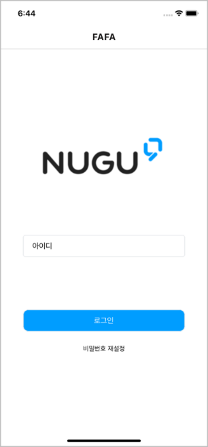
\includegraphics{images/f1.png}}
    \caption{Sign-in}
    \end{figure}
    \begin{enumerate}
        \item Client could sign-in with certified ‘username’\\
        URL : /login\\
	    METHOD : POST\\
        \item If certification is success, client get response data constitute of user’s role, latitude and longitude of home and company.\\
    \end{enumerate}
    \item Set location of home and company
    \begin{figure}[htbp]
    \centerline{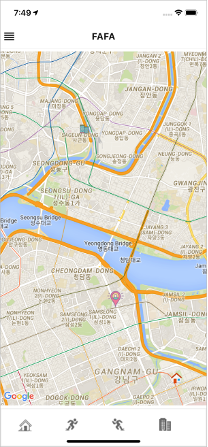
\includegraphics{images/f2.png}}
    \caption{Map}
    \end{figure}
    \begin{enumerate}
        \item Marker shows user’s current location\\
        \item Click house button on the bottom left, and your current location will be saved as your home. The home icon is displayed on the map.\\
        \item Click company button on the bottom right, and your current location will be save as your company. The company icon is displayed on the map.\\
        \item Send data to back-end server when Set home & company\\
        URL : /set\_location\\
        METHOD : POST
        \begin{table}[htbp]
        \caption{Request example of ‘set\_location’}
        \begin{center}
        \begin{tabular}{|c|c|}
        \hline
        Data     & example \\ \hline
        user.id  & 1       \\ \hline
        homeX    & 37.53820741       \\ \hline
        homeY    & 127.0310274        \\ \hline
        companyX & 37.555913728323375        \\ \hline
        companyY & 127.04942311226978        \\ \hline
        \end{tabular}
        \end{center}
        \end{table}
        \item Send data to back-end server when Alter home & company\\
        URL : /set\_location/user\_id \\
        METHOD : PUT/PATCH\\
    \end{enumerate}
    
    \item Update present location
    \begin{enumerate}
        \item Send recent location data to back-end server automatically every 100 meters using background function\\
    URL : /add\_location\\
    METHOD : POST
       \begin{table}[htbp]
       \caption{Request example of ‘add\_location’}
        \begin{center}
        \begin{tabular}{|c|c|}
        \hline
        Data     & example \\ \hline
        user.id  & 1       \\ \hline
        geoX    & 37.53820741       \\ \hline
        geoY    & 127.0310274        \\ \hline
        onHomeRoad & 0        \\ \hline
        onCompanyRoad &1       \\ \hline
        timeStamp&2020-12-08T17:18:44 \\ \hline
        \end{tabular}
        \end{center}
        \end{table}
        
    \end{enumerate}
    
    \item View kid’s request log
    \begin{figure}[htbp]
    \centerline{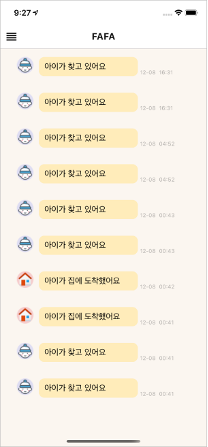
\includegraphics{images/f3.png}}
    \caption{View kid’s alert}
    \end{figure}
    
    \begin{enumerate}
        \item Get data from back-end server\\
	    URL : /alert\\
	    METHOD : GET
	    \begin{table}[htbp]
	    \caption{Matching of User’s intent and ‘alertType’}
	    \begin{center}
        \begin{tabular}{|c|c|}
        \hline
        alertType & Text in application \\ \hline
        0         & 아이가 찾고있어요.          \\ \hline
        1         & 아이가 집에 도착했어요.       \\ \hline
        \end{tabular}
        \end{center}
        \end{table}
    \end{enumerate}
\end{enumerate}

\subsection{Server}
\begin{enumerate}
    \item Judge parent’s location\\
    Server response different backend parameter to NUGU play depending on parent’s latest location.
    \begin{enumerate}
        \item Get parent’s latest location from ‘Location’ data table.
        \item Put the data in customized algorithm which use Machine Learning method. Random Forest is used to predict.
        
        \begin{figure}[htbp]
        \centerline{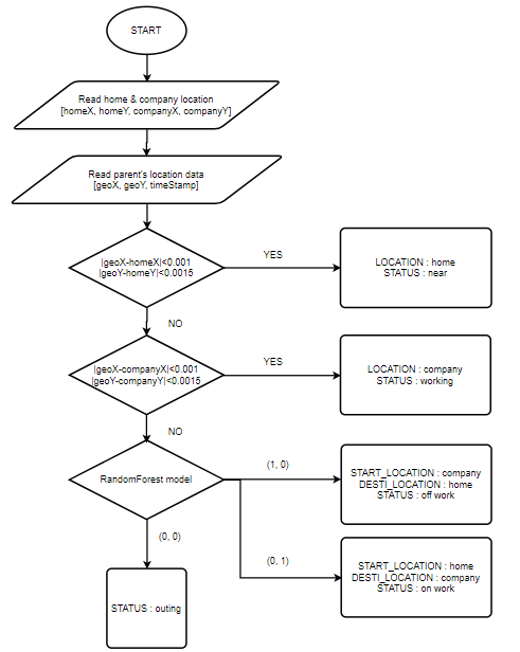
\includegraphics{images/f4.png}}
        \caption{VFlow of ‘Anlayze parent’s status based on location’}
        \end{figure}
        
        \item Response to NUGU play\\
    \end{enumerate}
    
    \item Save data to database
    \begin{enumerate}
        \item Django Framework handles to get data form NUGU play & Mobile application that we built.
        \item ) Save data in SQlite which is default option for Django. Django framework also handles this automatically.\\
    \end{enumerate}
    \item Make json for NUGU
    \begin{enumerate}
        \item Django Rest Framework module could handle this problem automatically using Serializers, JsonResponse module.\\
    \end{enumerate}
\end{enumerate}

\section{Architecture Design}
\subsection{Overall Architecture}
Our service is web-based application and heavily depends on Amazon Web Service for deployment. Our application’s UI is implemented with React Native. Server is implemented by Python with Django framework web server on it to serve data to frontend UI as REST API, and interact with SKTelecom NUGU’s API and speaker. Entire API server is running on Amazon Web Service EC2 instance.
\begin{figure}
    \centering
    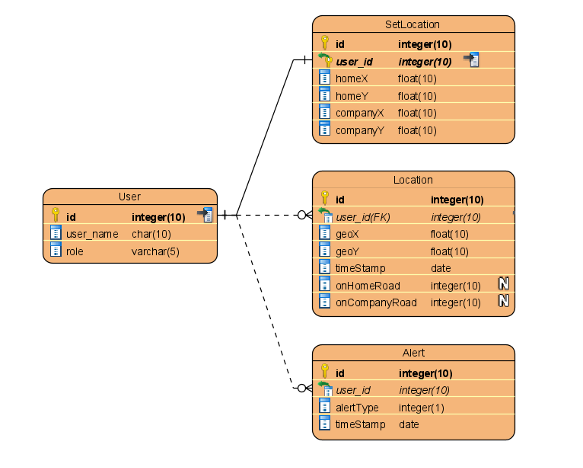
\includegraphics{images/f6.png}
    \caption{Entity Relationship Diagram}
\end{figure}

\begin{figure*}
    \centering
    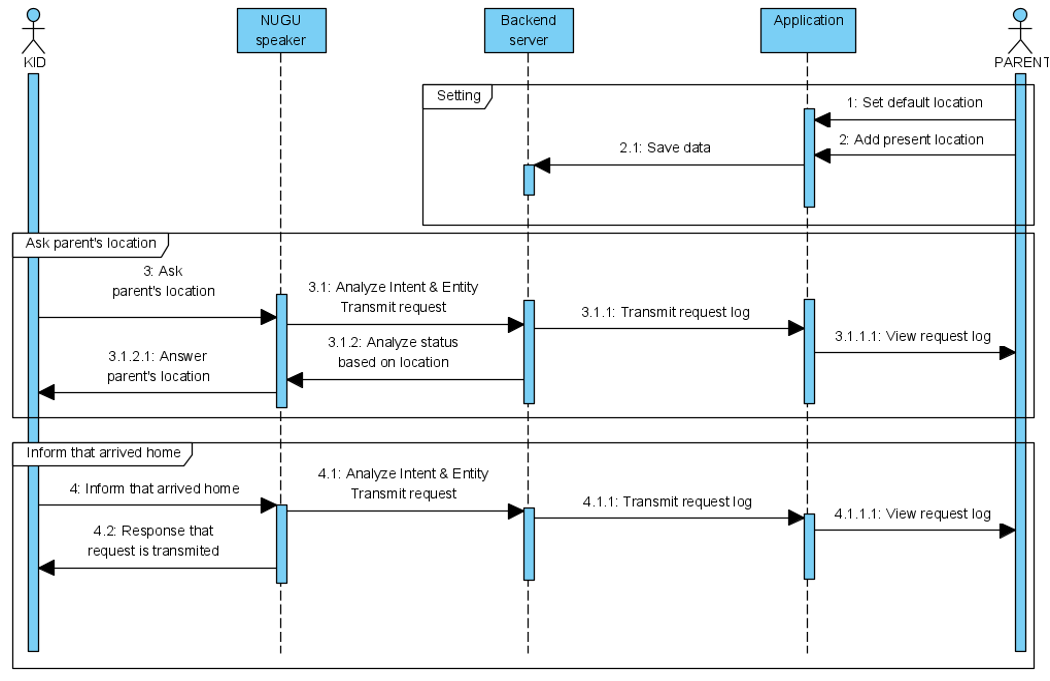
\includegraphics{images/f5.png}
    \caption{Sequence diagram}
\end{figure*}

\subsection{Database Design}
\begin{enumerate}
    \item User
    \begin{enumerate}
        \item id(PK) : identification of user
        \item user\_name : user’s name needed for sign-in
        \item role : role in family. To connect NUGU play and Application
    \end{enumerate}
    
    \item SetLocation
    \begin{enumerate}
        \item id(PK) : identification of SetLocation
        \item user\_id(FK) : reference ‘User’ table\\
        one user could set only one home and company
        \item homeX : longitude of user’s home
        \item homeY : latitude of user’s home
        \item companyX : longitude of user’s company
        \item companyY : latitude of user’s company
    \end{enumerate}
     
    \item Location
    \begin{enumerate}
        \item id(PK) : identification of Location
        \item user\_id(FK) : reference ‘User’ table\\
        one user could make multiple location logs
        \item geoX : lontitude of user’s latest location
        \item geoY : latitude of user’s latest location
        \item timeStamp : time of this data made
        \item onHomeRoad : To classify that user is on work
        \item onComapnyRoad : To classify that user is off work
    \end{enumerate}
    
    \item Alert
    \begin{enumerate}
        \item id(PK) : identification of Alert
        \item user\_id(FK) : reference ‘User’ table\\
	    one user could make multiple alert logs
	    \item alertType : define what request is this
	    \item timeStamp : time of this data made\\
    \end{enumerate}
\end{enumerate}

\subsection{Directory Organization – Front End}
Table 15 shows the directory organization of React-Native frontend application’s project.

\begin{table}[htbp]
\caption{DIRECTORY ORGANIZATION FOR \\FRONTEND APPLICATION PROJECT}
\begin{center}
\begin{tabular}{|c|c|c|}
\hline
Directory&File names  & Module name in use \\ \hline
 /src/components& Index.tsx &styled-components/native  \\ \hline
 /src/Assets/Images& .png &-  \\ \hline
/src/Screens/Navigator & Index.tsx& react-navigation \\ \hline
/src/Screens/Login &Index.tsx  & \begin{tabular}[c]{@{}c@{}}react-native-\\community/async-storage \end{tabular}\\  \hline
 /src/Screens/CheckLogin& Index.tsx  &\begin{tabular}[c]{@{}c@{}}react-native-\\community/async-storage \end{tabular}   \\ \hline
 /src/Screens/Map&Index.tsx  & \begin{tabular}[c]{@{}c@{}}react-native-maps,\\
react-native-geolocation-service
 \end{tabular}  \\ \hline
\end{tabular}
\end{center}
\end{table}

\begin{enumerate}
    \item /src/components\\
    React-native uses functional-component-based development method. This folder contains components that are frequently used like button, Input components. We will use these components by export and import function.\\
    \item /src/Assets/Images\\
    Inside the Asset folder, there are resources such as image files and fonts needed for the application. There are app icons, button images, and marker images in the image folder images.\\
    \item /src/Assets/Screens\\
    The Screens folder contains functions that make up the screens in the application. Navigator is a function that controls the movement of the screen. The screen consists of a Login screen for logins, a CheckLogin screen for tokens checking, and a Map window for positioning.\\
    \item styled-components/native\\
    Styled Components is an open-source library that helps with the application of styling of react and react native. It can create a style on a single JavaScript file. In other words, you can do CSS work in JavaScript files without CSS files.\\
    \item react-navigation\\
    A React Navigation is a chain of navigators that define the screen flow of your app. React Navigation's stack navigator provides a way for your app to transition between screens and manage navigation history.\\
    \item react-native-community/async-storage\\
    React Native Async Storage is an asynchronous, unencrypted, persistent, key-value storage system for React Native. Async Storage send and receive data like token, user information, location of home and company with Backend Server.\\
    \item react-native-geolocation-service\\
    React Native Geolocation Service tell user’s current location and allows to track user’s location. Using this module, we took user’s current location and whenever the user’s location changed, we used fetch module to send the location information to backend server.\\
    \item react-native-maps\\
    React Native Maps is a component system for maps. Using this module, we displayed Google Maps on the screen and marked house, company, user’s current location with marker\\
\end{enumerate}

\subsection{Directory Organization – Back End}

\begin{table}[htbp]
\caption{DIRECTORY ORGANIZATION FOR\\ BACKEND APPLICATION PROJECT}
\begin{center}
\begin{tabular}{|c|c|c|}
\hline
Directory&File names  & Module name in use \\ \hline
 /.ebextensions & django.config &\begin{tabular}[c]{@{}c@{}}Django,\\ AWS ElasticBeanstalk\end{tabular}   \\ \hline
 
/.elasticbeanstalk &config.yml & AWS ElasticBeanstalk  \\ \hline

/NUGU & \begin{tabular}[c]{@{}c@{}} settings.py, urls.py,\\ wsgi.py\end{tabular}&\begin{tabular}[c]{@{}c@{}} Django,\\ Django RestFramework \end{tabular}\\ \hline

/FAFA &\begin{tabular}[c]{@{}c@{}}models.py, serializers.py,\\ urls.py, views.py \end{tabular} & \begin{tabular}[c]{@{}c@{}} Django,\\ Django RestFramework \end{tabular}\\  \hline

 /static& .css, .js, .img,  &-   \\ \hline
 
 - & \begin{tabular}[c]{@{}c@{}} .gitignore, db.sqlite3,\\ manage.py, requirements.txt \end{tabular}&Django \\ \hline
\end{tabular}
\end{center}
\end{table}

\begin{enumerate}
    \item /.ebextensions\\
    In order to implement Django module on AWS ElasticBeanstalk environment, path configuration needed. ‘django.config’ file contains option for setting and covers deploy problem.\\
    \item /.elasticbeanstalk\\
    To upload directory on AWS instance, application name or region and the other configuration needed. ‘config.yml’ would cover upload problem.\\
    \item /NUGU\\
    In order to use Django framework which is run by Python, allowed hosts, url, apps, packages and other things should be set on this directory. On ‘settings.py’ and ‘urls.py’ files, there are some customized setting for this project.\\
    \item /FAFA\\
    Django RestFramework module is used in this directory. ‘models.py’ make models (DB table). ‘urls.py’ handles routing. ‘views.py’ gets request and sends response by function that we made. ‘serializers.py’ make response in json form from queryset.\\
    \item SQLite \\
    SQLite is relatively light embedded database for applications. To store data, only one file ‘db.sqlite3’ is needed. Small and concise DB would run in local, so you don’t have to worry about the cost of network configuration, firewalls, network address translation, and so on. We can only focus on code level.\\
    \item AWS ElasticBeanstalk\\
    A fully managed service of AWS that deploy, expand and manage web application. It handles capacity provisioning, load balancing, auto-scaling, monitoring, and hosting environment automatically. So user just deploy application. In addition, there is no unnecessary expenditure to pay. Through easy deployment, this module makes us focus on code level during development. \\
    \item Django\\
    Django is Web framework used in our project. Using this module, we don’t ‘reinvent the wheel’ about HTTP service. Django provide simple and convenient middle-ware like routing, error-handler and parser. Many of above middle-ware can be implemented in custom way that we want to make.\\
    \item Django Rest Framework(DRF)\\
    DRF is a powerful and flexible module for creating WEB APIs. To develop back-end proxy server of NUGU-PLAY in REST API form, we used DRF. This module has powerful ‘viewset’ that enables us to develop CRUD functions easily and quickly. Also, we can customize a general view. \\
    \item sklearn.ensemble\\
    The sklearn.ensemble module includes two averaging algorithms based on randomized decision trees: the RandomForest algorithm and the Extra-Trees method. Both algorithms are perturb-and-combine techniques specifically designed for trees. This means a diverse set of classifiers is created by introducing randomness in the classifier construction. The prediction of the ensemble is given as the averaged prediction of the individual classifiers.\\
\end{enumerate}

\section{Use Cases}
FAFA service is used by kids and parents. Kids use our service via NUGU speaker, parents use our service throguh application that we developed in React Native. Application and NUGU speaker are connected by backend proxy server which is developed in REST API form by Django framework. Under Diagram shows flow of our service and algorithm that how to define parent’s status based on location data.
\subsection{AI speaker}
Depending on above algorithm which is using Machine Learning to define that parents are on-work or off-work, There are 3 answers when kids ask parent’s location through NUGU speaker. In addition, there is a fixed response when inform to speaker that kids arrived home.\\
\begin{figure}[htbp]
    \centering
    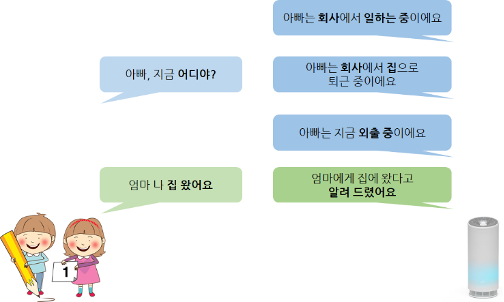
\includegraphics{images/f7.png}
    \caption{AI speaker VUI}
\end{figure}

\begin{enumerate}
    \item Ask “엄마, 지금 어디야?”\\
    Kids ask to AI speaker “Mom, Where are you now?”
    SKTelcom’s NUGU play analyze user’s intent and entity. Then, request parent’s current location information to back-end proxy server.\\
    \item Answer “엄마는 회사에 있어요” \\
    If parent’s latest location is near to home or office, NUGU speaker tells to kids “Mom is working in office” or “Fafa is near home”. Figure 10 explains this logic. 0.001 longtitude means 100 meter and 0.0015 longtitude means 100 meter.\\
    \item Answer “아빠는 회사에서 집으로 퇴근하는 중이에요”\\
    We predict parent’s status by using randomForest which is one of Machine Learning method. Train data is saved automatically by application that we made. If kids ask parent’s location, backend server puts parent’s latest location on randomForest model and judge that parents are coming or going home. \\
    \item Answer “아빠는 외출 중이에요”\\
    If parent’s latest location is out of boundary between home and company. NUGU speaker says “Parent is out now”\\
    \item Inform “엄마, 저 집 도착했어요”\\
    Kids ask to AI speaker “Mom, I arrived home now”
    SKTelcom’s NUGU play analyze user’s intent and entity. Then, this request is saved as log in database through back-end server.\\
    \item Answer “엄마에게 집에 도착했다고 알려 드렸어요” \\
    If kids inform that they arrived home now, NUGU speaker sends this log to backend server and response above message.\\
\end{enumerate}

\subsection{Application}
\begin{enumerate}
    \item Sign-in\\
    \begin{figure}[htbp]
    \centering
    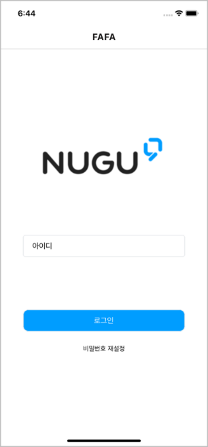
\includegraphics{images/f8.png}
    \caption{Sign-in}
    \end{figure}\\
    When user access our application, They have to login by ID(user name)\\
    
    \item Landing page\\
    \begin{figure}[htbp]
    \centering
    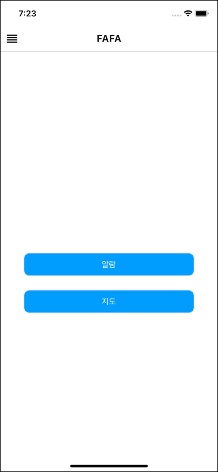
\includegraphics{images/f9.png}
    \caption{Landing}
    \end{figure}\\
    When user log in to our application, the landing screen is on. There are two options. One is an alarm page that shows alarm and the other is a map page that track user’s location.\\
    
    \item View Alert page\\
    \begin{figure}[htbp]
    \centering
    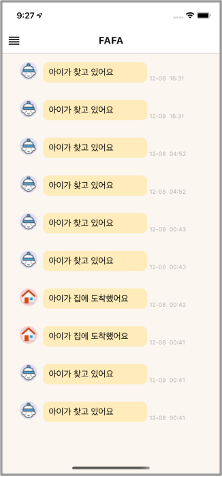
\includegraphics{images/f10.png}
    \caption{View Kid’s request}
    \end{figure}\\
    This page shows that when the kids found his parents and when informed that they arrived home through AI speaker. It informs notification and the time.\\
    
    \item Map Page\\
    \begin{figure}[htbp]
    \centering
    \hfill
    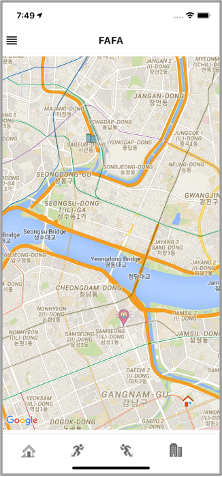
\includegraphics{images/f11.png}
    \hfill
    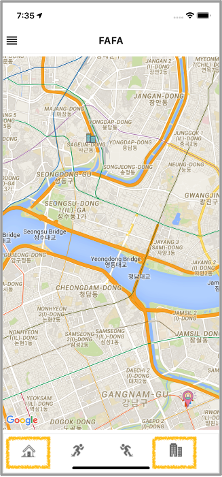
\includegraphics{images/f11-2.png}
    \caption{Set Home \& Company location}
    \end{figure}
    
    Markers shown above Google Map indicate your current location. On 100m movement, the current location is automatically transferred to the server.\\ \\
    Click the Home/Company icon at the bottom to save the current user’s location to the location of home or company.\\
    \begin{figure}[htbp]
    \centering
    \hfill
    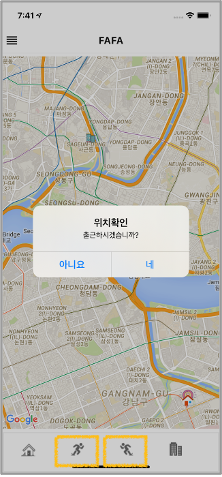
\includegraphics{images/f12-1.png}
    \hfill
    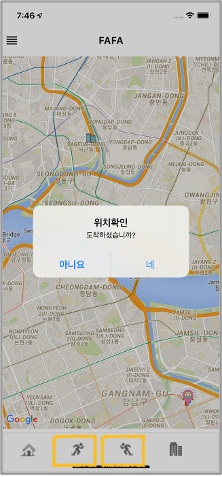
\includegraphics{images/f12-2.png}
    \caption{Test data for Machine Learning }
    \end{figure}\\
    Click the bottom button before and after work.\\
    Through this function, the commuting route and time are analyzed using machine learning techniques.\\
    When enough data is available, it automatically recognizes commuting information without having to click the button and informs your child of the parent's location.

\end{enumerate}
\end{document}
